\documentclass{article}
\usepackage{amsmath}
\usepackage{graphicx}
\begin{document}
\section{Execute}
\subsection{Circuit Diagram}
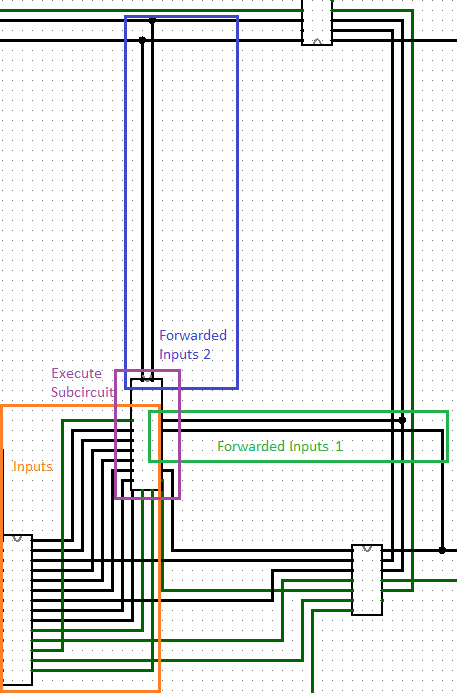
\includegraphics[width=8cm]{ALU.png}
\\
Our execute stage is all condensed into one subcircuit (with additional lower level circuits within the subcircuit). The subcircuit gets its inputs mainly from the ID/EX registers but also from the EX/MEM and MEM/WB registers for use in the forwarding unit. The two outputs of the subcircuit is the main output C, and the Write Enable for the Register File. 

The Execute subcircuit has many subcircuits of its own. For each of the main inputs, A and B, with respective register addresses rs and rt, there is a forwarding unit that resolves data hazard issues that are present in this Mini-Mips processor. There is a multiplexor for B that chooses between B and the immediate. There are special sections that implement the SLT, SLTI, SLTIU, SLTU, and the MOVZ, MOVN commands as well. There are a few multiplexors that choose between several possible outputs depending on the MIPS command.

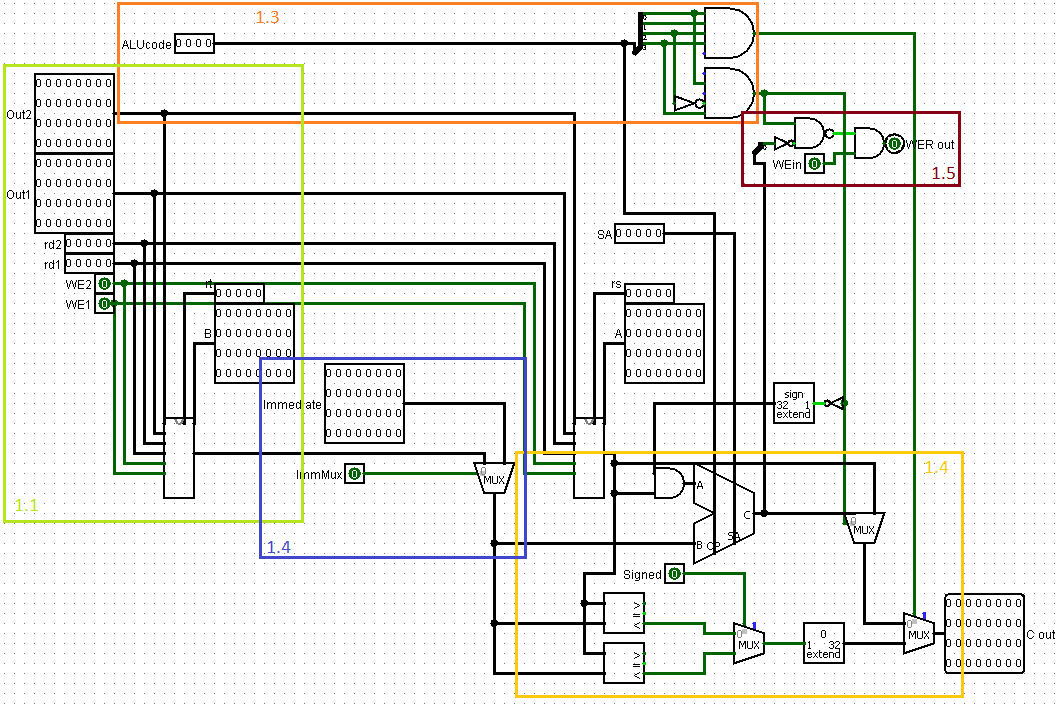
\includegraphics[width=17cm]{EXOVER.png}

\subsubsection{Forwarding Unit}
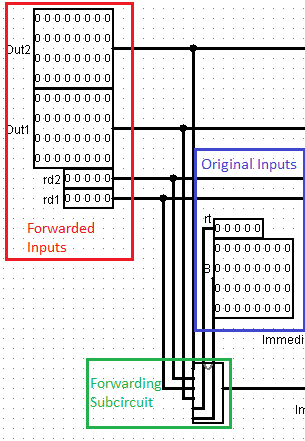
\includegraphics{Forward1.png}
This part of the circuit compares the register address (rs) of a main input (Out0) with the write destinations of the instruction in the next stage (rd1) and the stage after that (rd2). Out1 and Out2 are to be written in those destinations respectively. The Forwarding Unit takes these 6 inputs and chooses one of the 3 32-bit outputs Out0, Out1, Out2. Figure 3b shows the location of the Forwarding Unit in the Execute circuit for input B. 

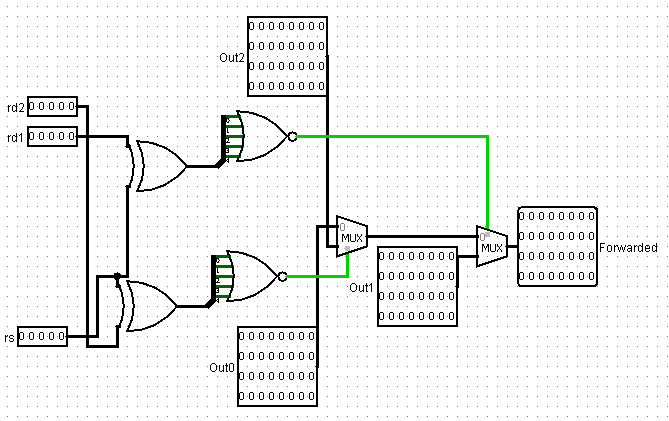
\includegraphics{Forward2.png}
The Forwarding Unit compares the register addresses using an XOR and a NOR gate, to get a multiplexor selector, that is, if the register addresses are equal, we get 1, and otherwise 0. This is done for each rs and rd1, and rs and rd2. We first choose between Out0 and Out2 by comparing rs and rd2, then the selected and Out1 by comparing rs and rd1. This process automatically gives Out1 higher priority than Out2; if all of rs, rd1, and rd2 are equal, Out1 will be chosen over Out2. 

\subsubsection{Immediate Mux}
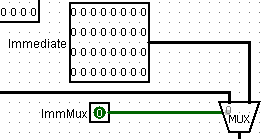
\includegraphics{Immediate.png}
This small section of the Execute circuit just chooses between Immediate and the second main input B. The Immediate is already bit extended to 32 bits, and our Decoder gives us a multiplexor selector bit ImmMux that we use here. 

\subsubsection{Special Command Determination}
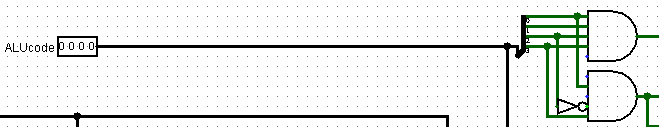
\includegraphics{Code.png}
These 2 and gates explictly look for certain ALU Op codes. The Op code 1111 identifies the command as one of the SLT commands while the Op code 1x01 identifies the command as MOVN or MOVZ. We use these bits specially for executing these commands correctly in other parts of the circuit.

\subsubsection{Outputs}
\includegraphics{OUTPUT.png}
The output C out is by default rooted from the output C from the ALU. However, there are 2 multiplexors, M1 and M2, that select for the final output of the subcircuit. M1 corresponds to the commands MOVN and MOVZ; that is, if the ALU Op code is 1x01, the output will be the first main input A (after corrected by the forwarding unit) instead of the output C from the ALU. M3 corresponds to the commands SLT, SLTI, SLTU, SLTIU; that is, if the ALU Op code is 1111, the output will be determined in the section labeled SLT in the figure. 
\begin{itemize}
\item
SLT: We use two comparators to do the SLT commands. For SLTU and SLTIU, we use the upper unsigned comparator, and for SLT and SLTI, we use the lower 2's complement comparator. We choose between the two outputs at multiplexor Y with a bit indicating whether the comparison is signed or not, Signed. Then the 1 bit output is sign extended to 32 bits. 

\item
X: For the MOVN and MOVZ commands, we are comparing B against 0 instead of A. The lower input to the AND gate labeled X is just the original input coming from the Forwarding Unit. The upper input to X is either 32-bits of all 0's if the ALU Op code is 1x01 or all 1's otherwise. The wire leading out of X is therefore all 0's if the command is MOVN or MOVZ, and the original input otherwise.

\end{itemize}
\subsubsection{Write Enable for MOV}
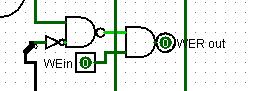
\includegraphics{MOV.png}
The final piece of the circuit deals with the MOVN and MOVZ commands. Since these two only write based on the given condition, we modify the write enable (WE in) if the condition was not met and the command was MOVN or MOVZ to begin with. In our implementation, the lower lead in to the NAND gate is the truth value of the condition, coming from the ALU (negated), and the upper lead in indicates whether or not the command is MOVN or MOVZ. As such, the output of the NAND gate is true if either the command is not MOVx, or if the condition was true. 

\subsection{Correctness Constraints}
\begin{itemize}
\item The correctness of this module depends on the correctness of the inputs that are decoded in the Instruction Decode stage. Therefore, one functional requirement is that the inputs are consistent with the MIPS command given. For instance, WE in (write enable) must be 1 if the command ultimately writes back to the Register File. 
\item The module takes inputs from the Memory and Write Back Stages. Therefore, these stages need to be implemented correctly in order for this stage to be correct.
\item The execute subcircuit in this implementation is only correct for the instructions in Table A, and pseudo correct (set as NOPs) for the instructions in Table B. Only these instructions can be given in the Instruction Fetch Stage.

\end{itemize}

\subsection{Testing}
A large portion of the instructions depend on the correctness of the ALU circuit. Since that is given to us, we assume its correctness. For those instructions, computation is given correct, so we only have to test one case for each, that is, if one case gives us the correct nontrivial output (like 0 or something that could have been an accident), then the data path was correct and all inputs for that instruction should give us a correct output. 

There are 6 functions that are not computed using the ALU: SLT, SLTU, SLTI, SLTIU, MOVN, and MOVZ. These need to 
\end{document}